\documentclass[12pt,a4paper]{article}

\usepackage[T1]{fontenc}

\usepackage[fleqn]{amsmath} % This package with the fleqn option aligns equations to the left
\setlength{\mathindent}{0pt} % Set indentation from the left margin

\usepackage{amssymb} % Required for math symbols
\usepackage{graphicx} % Required for inserting images
\usepackage{geometry}

\usepackage{longtable}
\usepackage{subcaption}

\usepackage[backend=biber, style=authoryear, citestyle=authoryear]{biblatex}
\addbibresource{references.bib}

\geometry{a4paper, margin=1in}

{
\title{
    
\includegraphics[width=0.33\textwidth]{/Users/mlnick/Documents/Images/tsukuba-logo.png} \\
    \vspace{3mm}  
    \textbf{Practical Development for IoT and Embedded Systems} \\
    \vspace{3mm}    
    Report 1 on the Individual Application Project
}

\author{Mamanchuk Mykola, SID.202420671}
\date{\today}
}

\usepackage{listings}
\usepackage{color}

\definecolor{codegreen}{rgb}{0,0.6,0}
\definecolor{codegray}{rgb}{0.5,0.5,0.5}
\definecolor{codepurple}{rgb}{0.58,0,0.82}
\definecolor{backcolour}{rgb}{0.99,0.99,0.99}

\lstdefinestyle{mystyle}{
    backgroundcolor=\color{backcolour},   
    commentstyle=\color{codegreen},
    keywordstyle=\color{magenta},
    numberstyle=\tiny\color{codegray},
    stringstyle=\color{codepurple},
    basicstyle=\ttfamily\footnotesize,
    breakatwhitespace=false,         
    breaklines=true,                 
    captionpos=b,                    
    keepspaces=true,                 
    numbers=left,                    
    numbersep=5pt,                  
    showspaces=false,                
    showstringspaces=false,
    showtabs=false,                  
    tabsize=2
}
\lstset{style=mystyle}

\begin{document}

\maketitle

\section{Introduction}

\subsection{Application Description}

The \textbf{AlcoTester} application is designed with a humorous touch, intended to be funny among friends. The idea stems from the observation that a person, especially when drunk, might not quickly understand the sequence of events in the test. Imagine the following scenario: you start the test and hand the phone to your friend. Confused and possibly intoxicated, your friend changes the position of the phone during the accelerometer test. Next, during the voice test, there is a high likelihood of your friend altering his voice due to inebriation. Although this situation is somewhat silly, it highlights the fun aspect of the application.

While the primary purpose of the application is to entertain, it also serves a functional role in assessing a person's sobriety. However, it is important to note that the current version of the application requires further development to confidently catch a person who is drunk. If you are alone, it is still not recommended to solely rely on this application to test your sobriety. In cases where you are unsure of your state, this application can provide an independent assessment to help you make an informed decision.

The complete listing source for the application can be accessed following the reference [1].

\subsection{Development Environment}
The \textbf{AlcoTester} application was developed using \textit{Android Studio} on a Windows 11 Pro system with an Intel Core i7-1185G7 processor. The device used for testing the application was a Nexus 7.

\section{How to Use}

The UI is designed to be simple and intuitive to avoid user confusion. Once the user starts the test, the data recording begins with the accelerometer, followed by the voice data. The interface shows the progress of the recordings, and the results are displayed as a probability of drunkenness.

\begin{enumerate}
    \item \textbf{Start Screen:} Launch the app and press the "Begin Test" button.
    \item \textbf{Accelerometer Recording:}
    \begin{itemize}
        \item Press "Record Data".
        \item Follow on-screen instructions to hold the device steady for 10 seconds.
    \end{itemize}
    \item \textbf{Voice Recording:}
    \begin{itemize}
        \item Press "Record Voice".
        \item Speak a sentence into the microphone for 5 seconds.
    \end{itemize}
    \item \textbf{Analyze Results:}
    \begin{itemize}
        \item Press "Analyze Results" to process the recorded data.
        \item View the displayed percentage likelihood of being drunk.
    \end{itemize}
\end{enumerate}

\newpage

\section{Screenshots}

\begin{figure}[htb!]
    \centering
    \begin{subfigure}[b]{0.35\textwidth}
        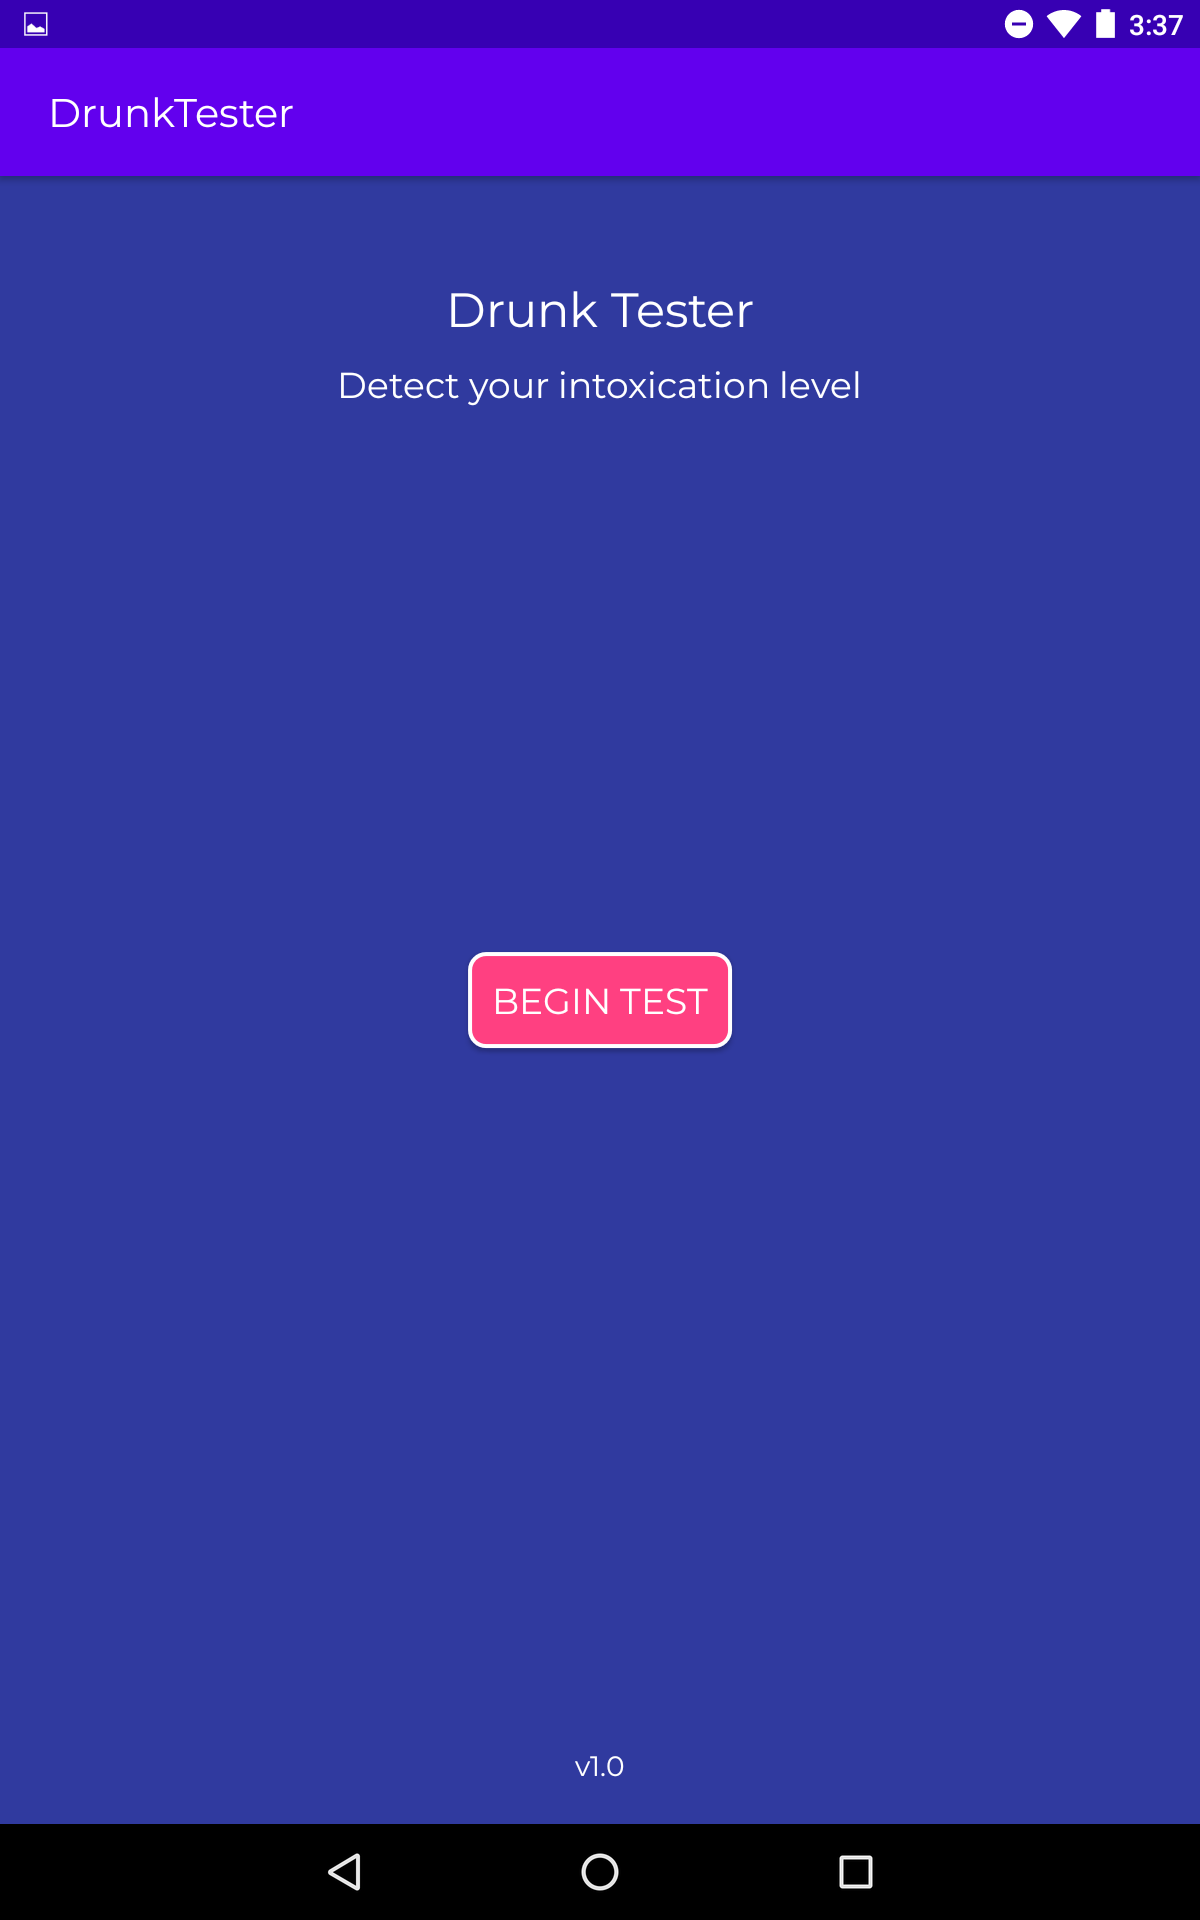
\includegraphics[width=\textwidth]{materials/Start_screen.png}
        \caption*{Start Screen: The initial screen of the Drunk Tester application.}
    \end{subfigure}
    \hfill
    \begin{subfigure}[b]{0.35\textwidth}
        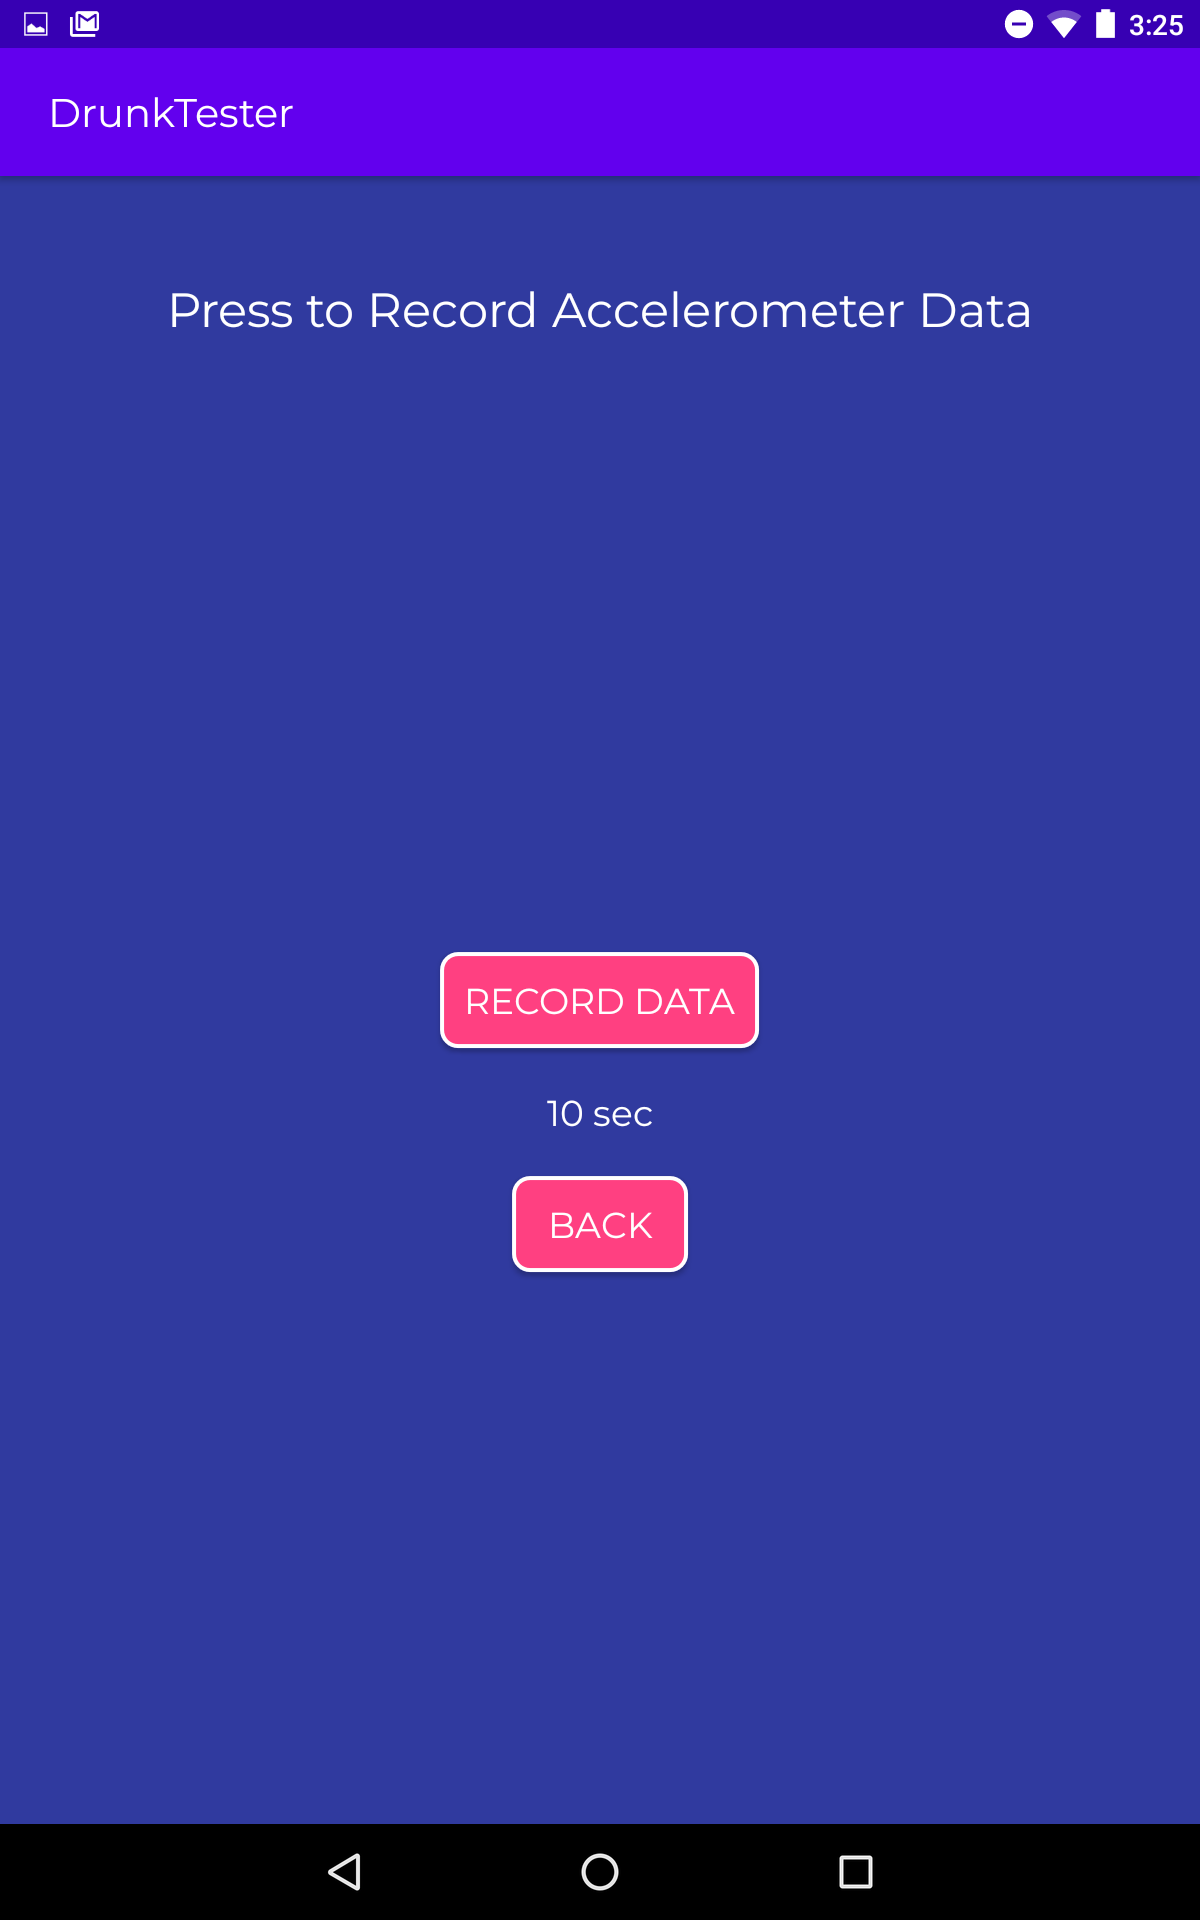
\includegraphics[width=\textwidth]{materials/Press_to_record_accelerometer_data.png}
        \caption*{Press to Record Accelerometer Data: The screen instructing the user to record accelerometer data.}
    \end{subfigure}
\end{figure}

\begin{figure}[htb!]
    \begin{subfigure}[b]{0.35\textwidth}
        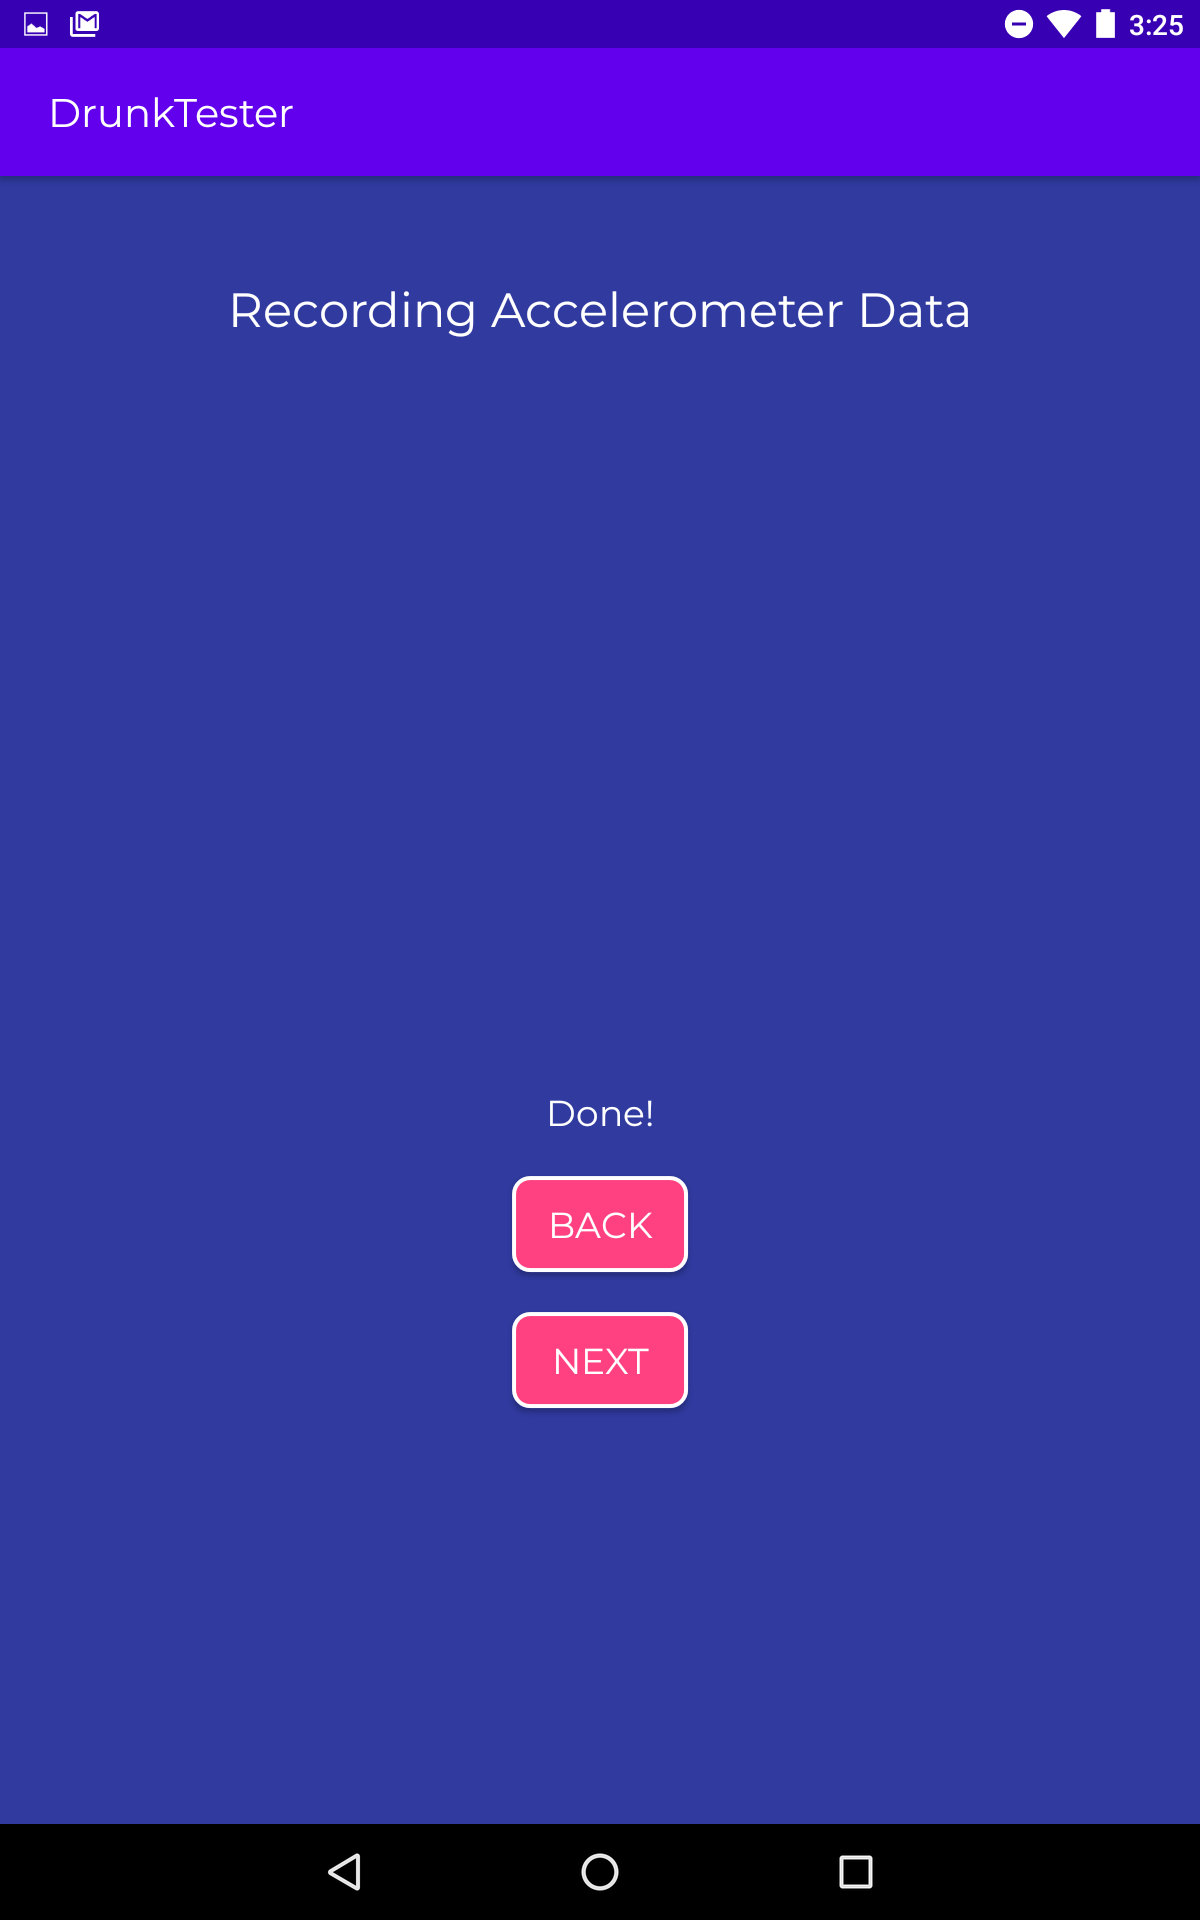
\includegraphics[width=\textwidth]{materials/Recording_accelerometer_data_done.png}
        \caption*{Recording Accelerometer Data: Progress screen showing the recording of accelerometer data.}
    \end{subfigure}
    \hfill
    \begin{subfigure}[b]{0.35\textwidth}
        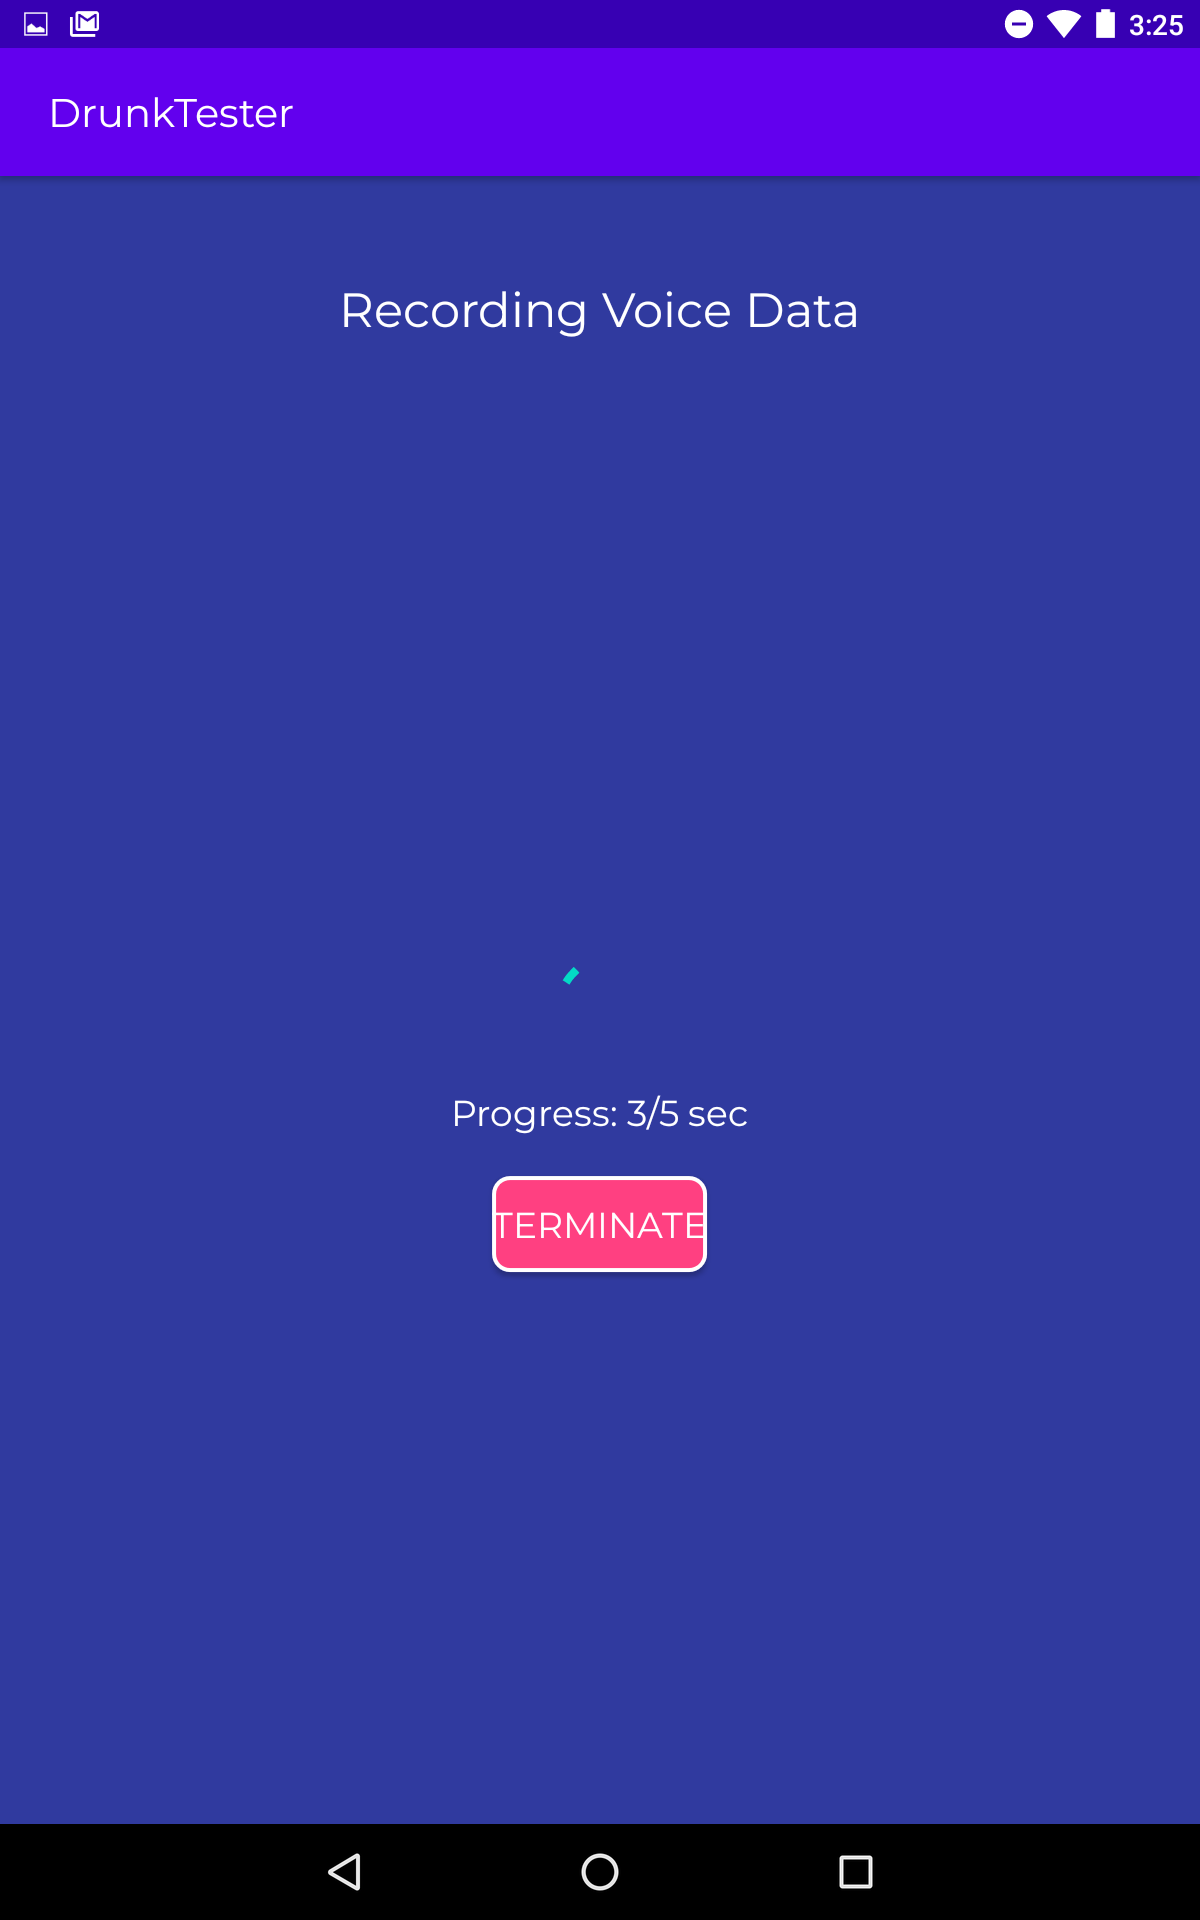
\includegraphics[width=\textwidth]{materials/Recording_voice_data.png}
        \caption*{Press to Record Voice Data: The screen instructing the user to record voice data.}
    \end{subfigure}
\end{figure}

\newpage

\begin{figure}[htb!]
    \begin{subfigure}[b]{0.35\textwidth}
        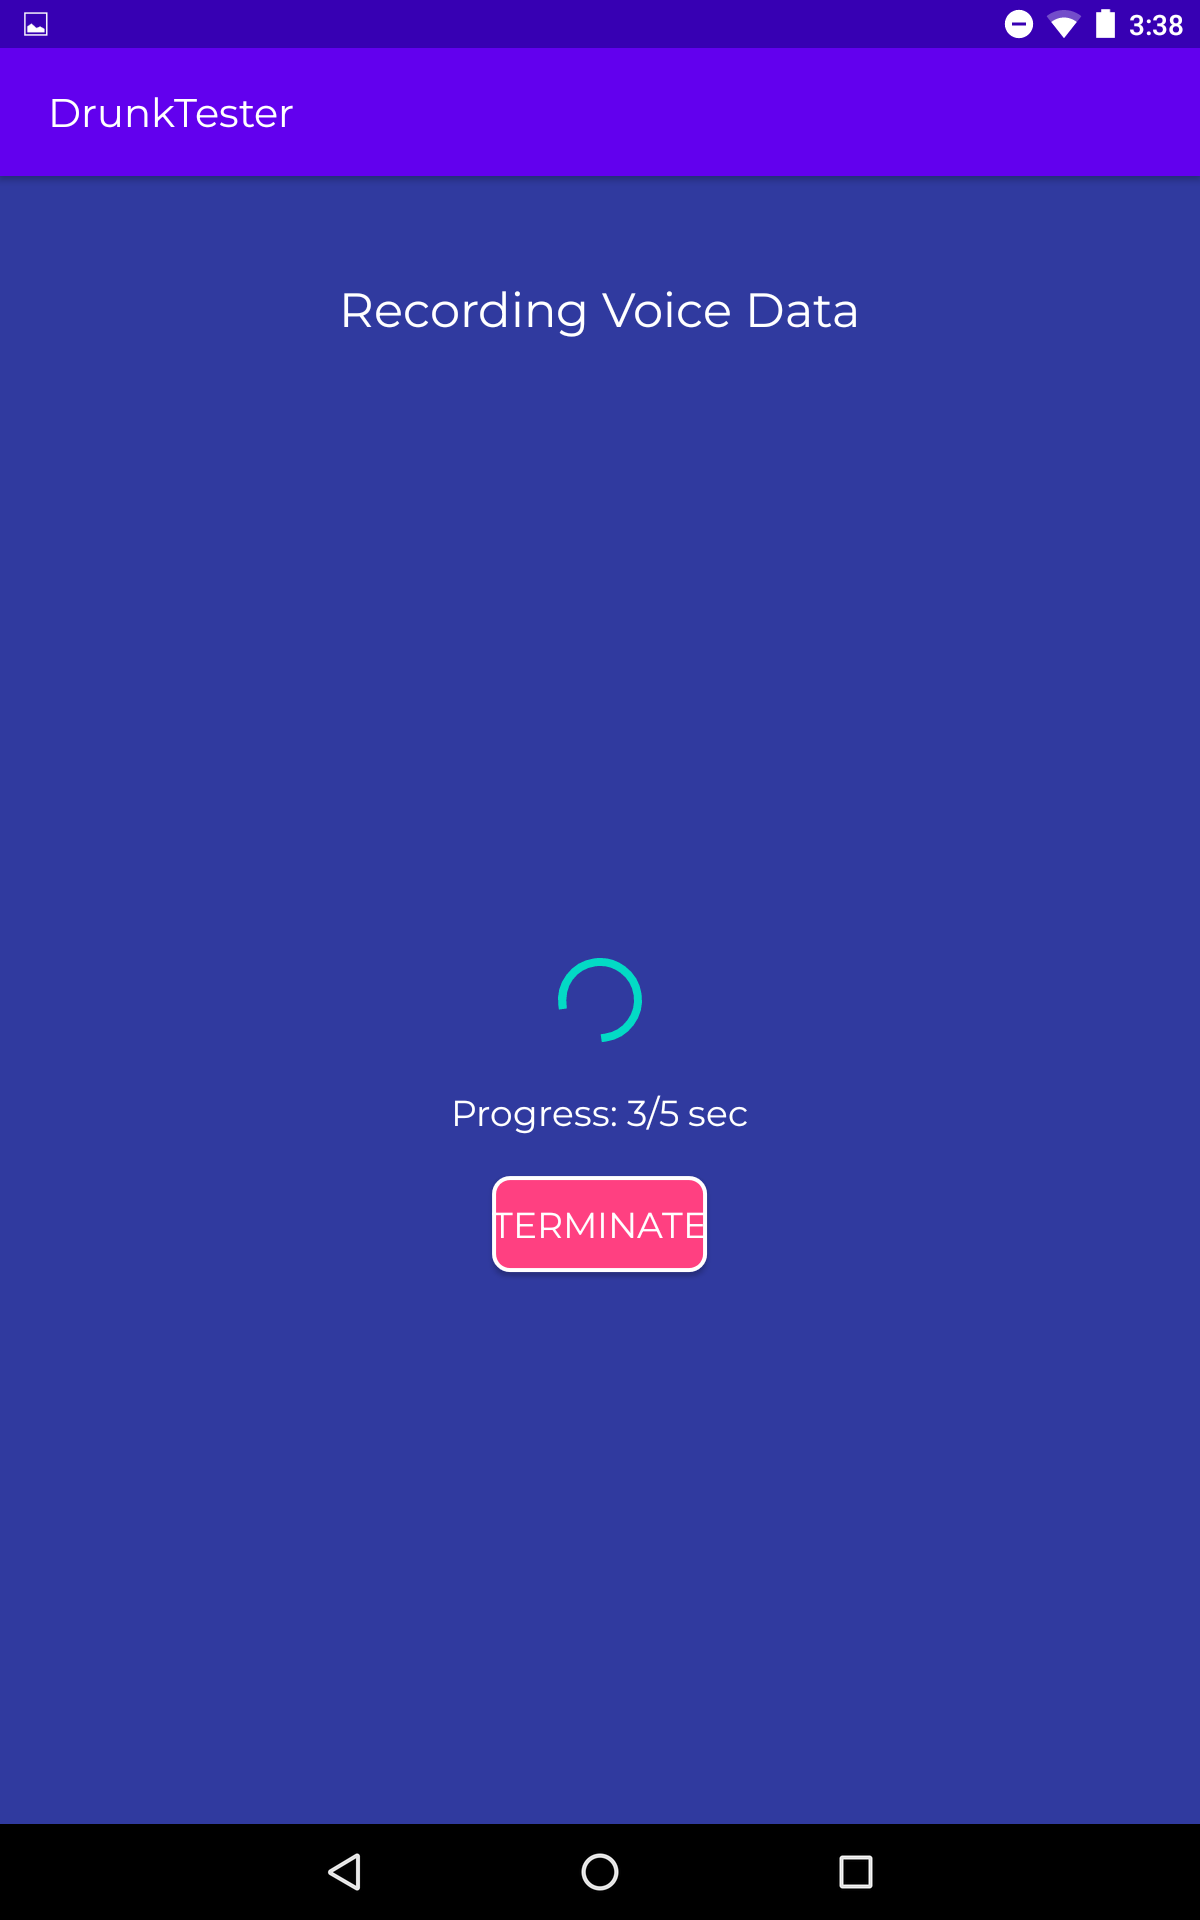
\includegraphics[width=\textwidth]{materials/Recording_voice_data_2.png}
        \caption*{Recording Voice Data: Progress screen showing the recording of voice data.}
    \end{subfigure}
    \hfill
    \begin{subfigure}[b]{0.35\textwidth}
        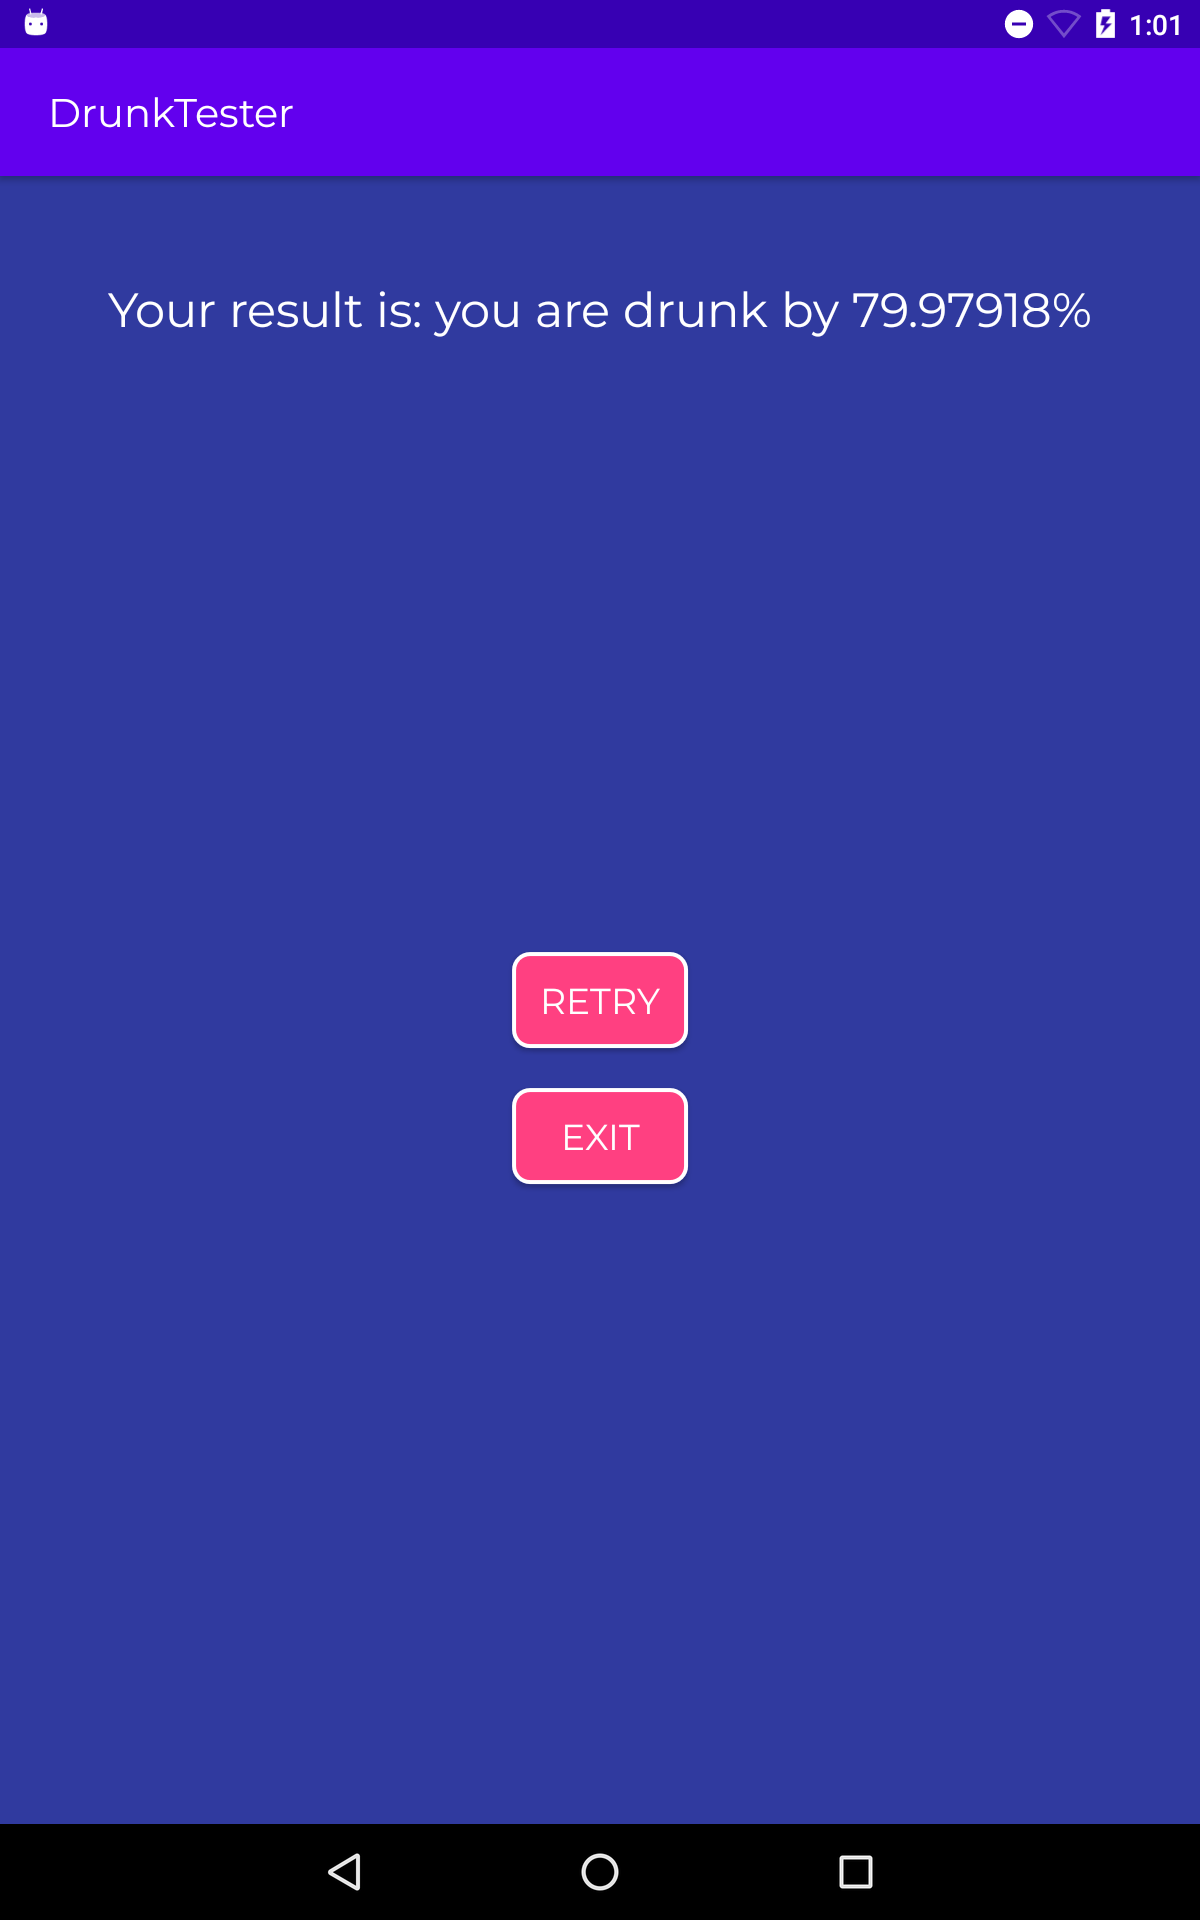
\includegraphics[width=\textwidth]{materials/Result_showcase.png}
        \caption*{Result Showcase: The screen displaying the result of the drunk test.}
    \end{subfigure}
\end{figure}

\begin{figure}[htb!]
    \begin{subfigure}[b]{0.35\textwidth}
        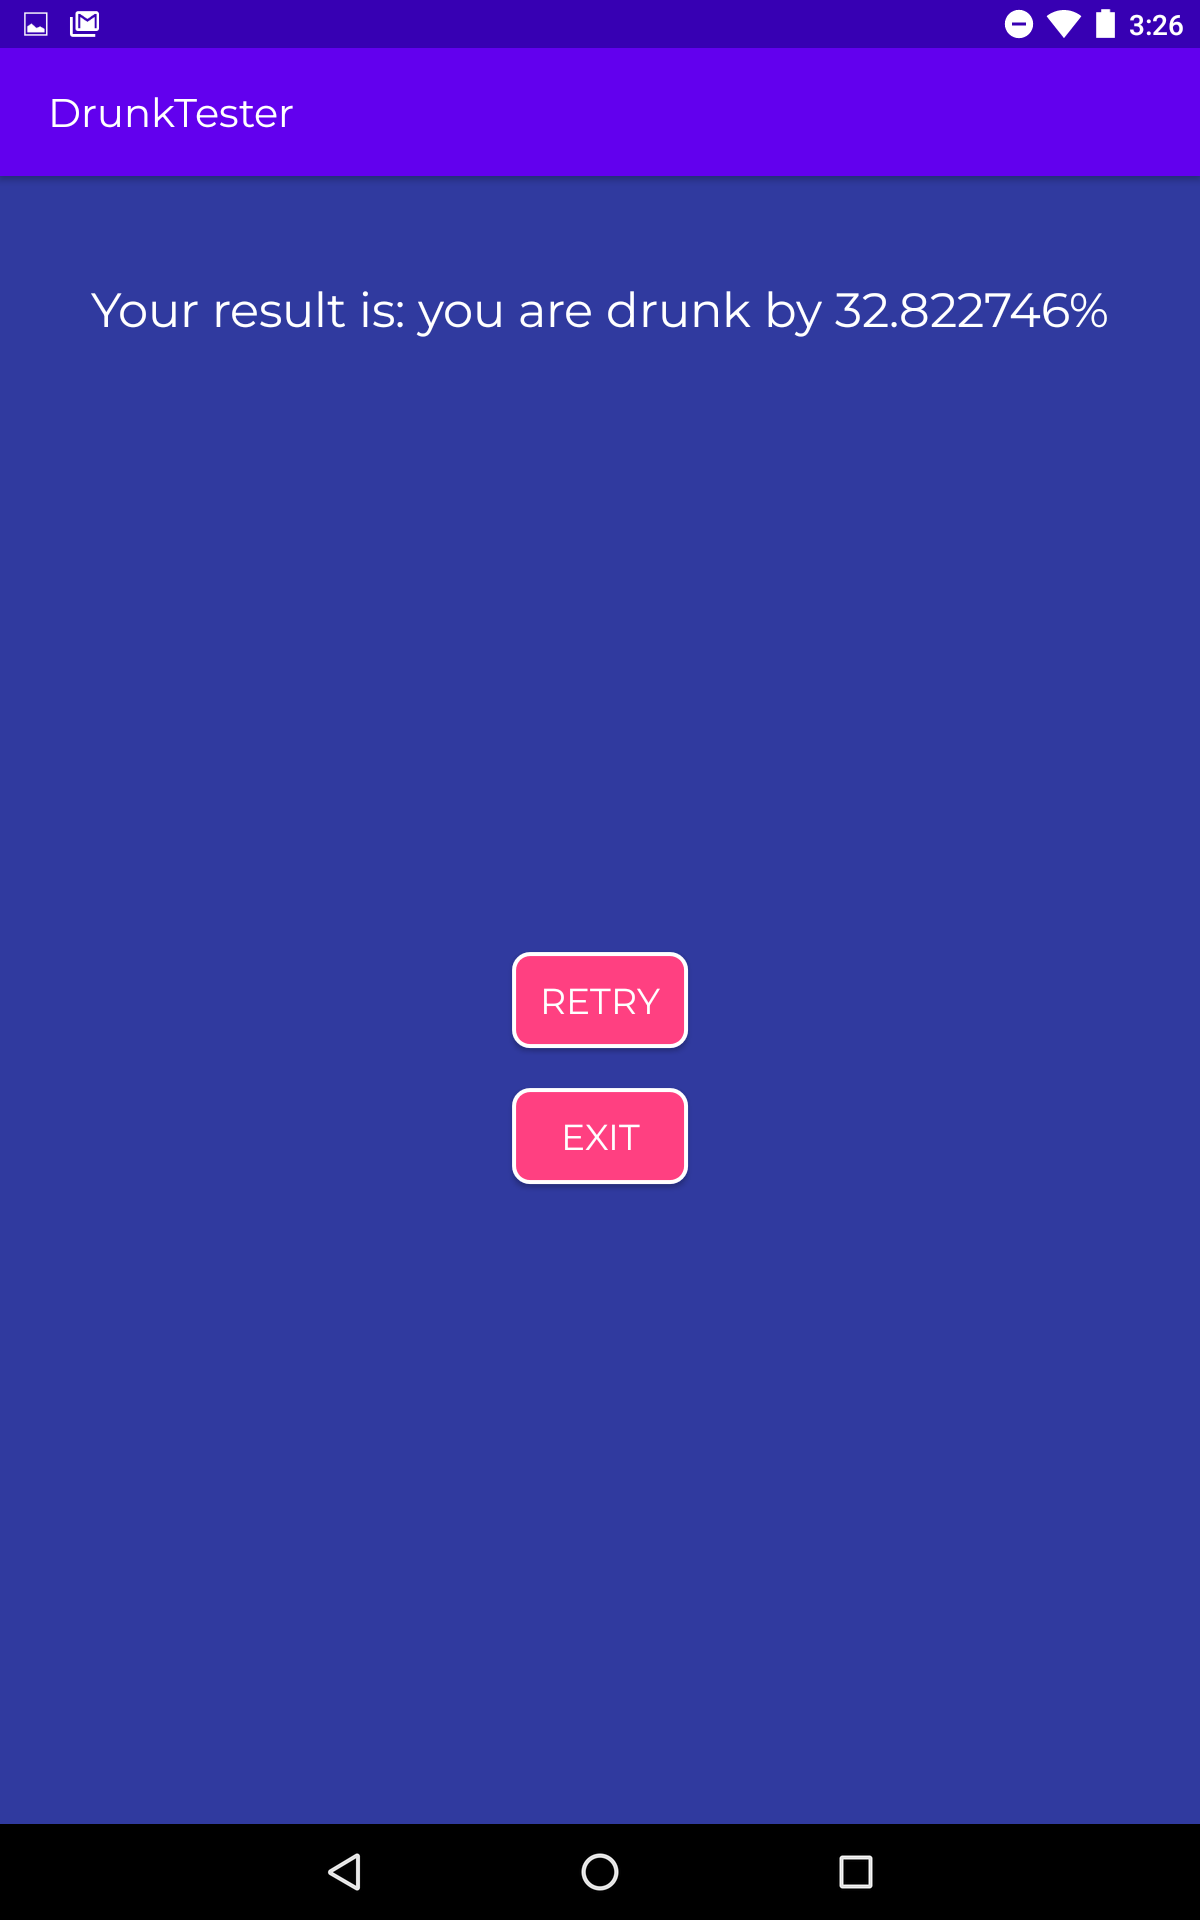
\includegraphics[width=\textwidth]{materials/Showcase_result_low.png}
        \caption*{Result Showcase Low: The screen displaying a lower percentage of being drunk.}
    \end{subfigure}
    \hfill
    \begin{subfigure}[b]{0.35\textwidth}
        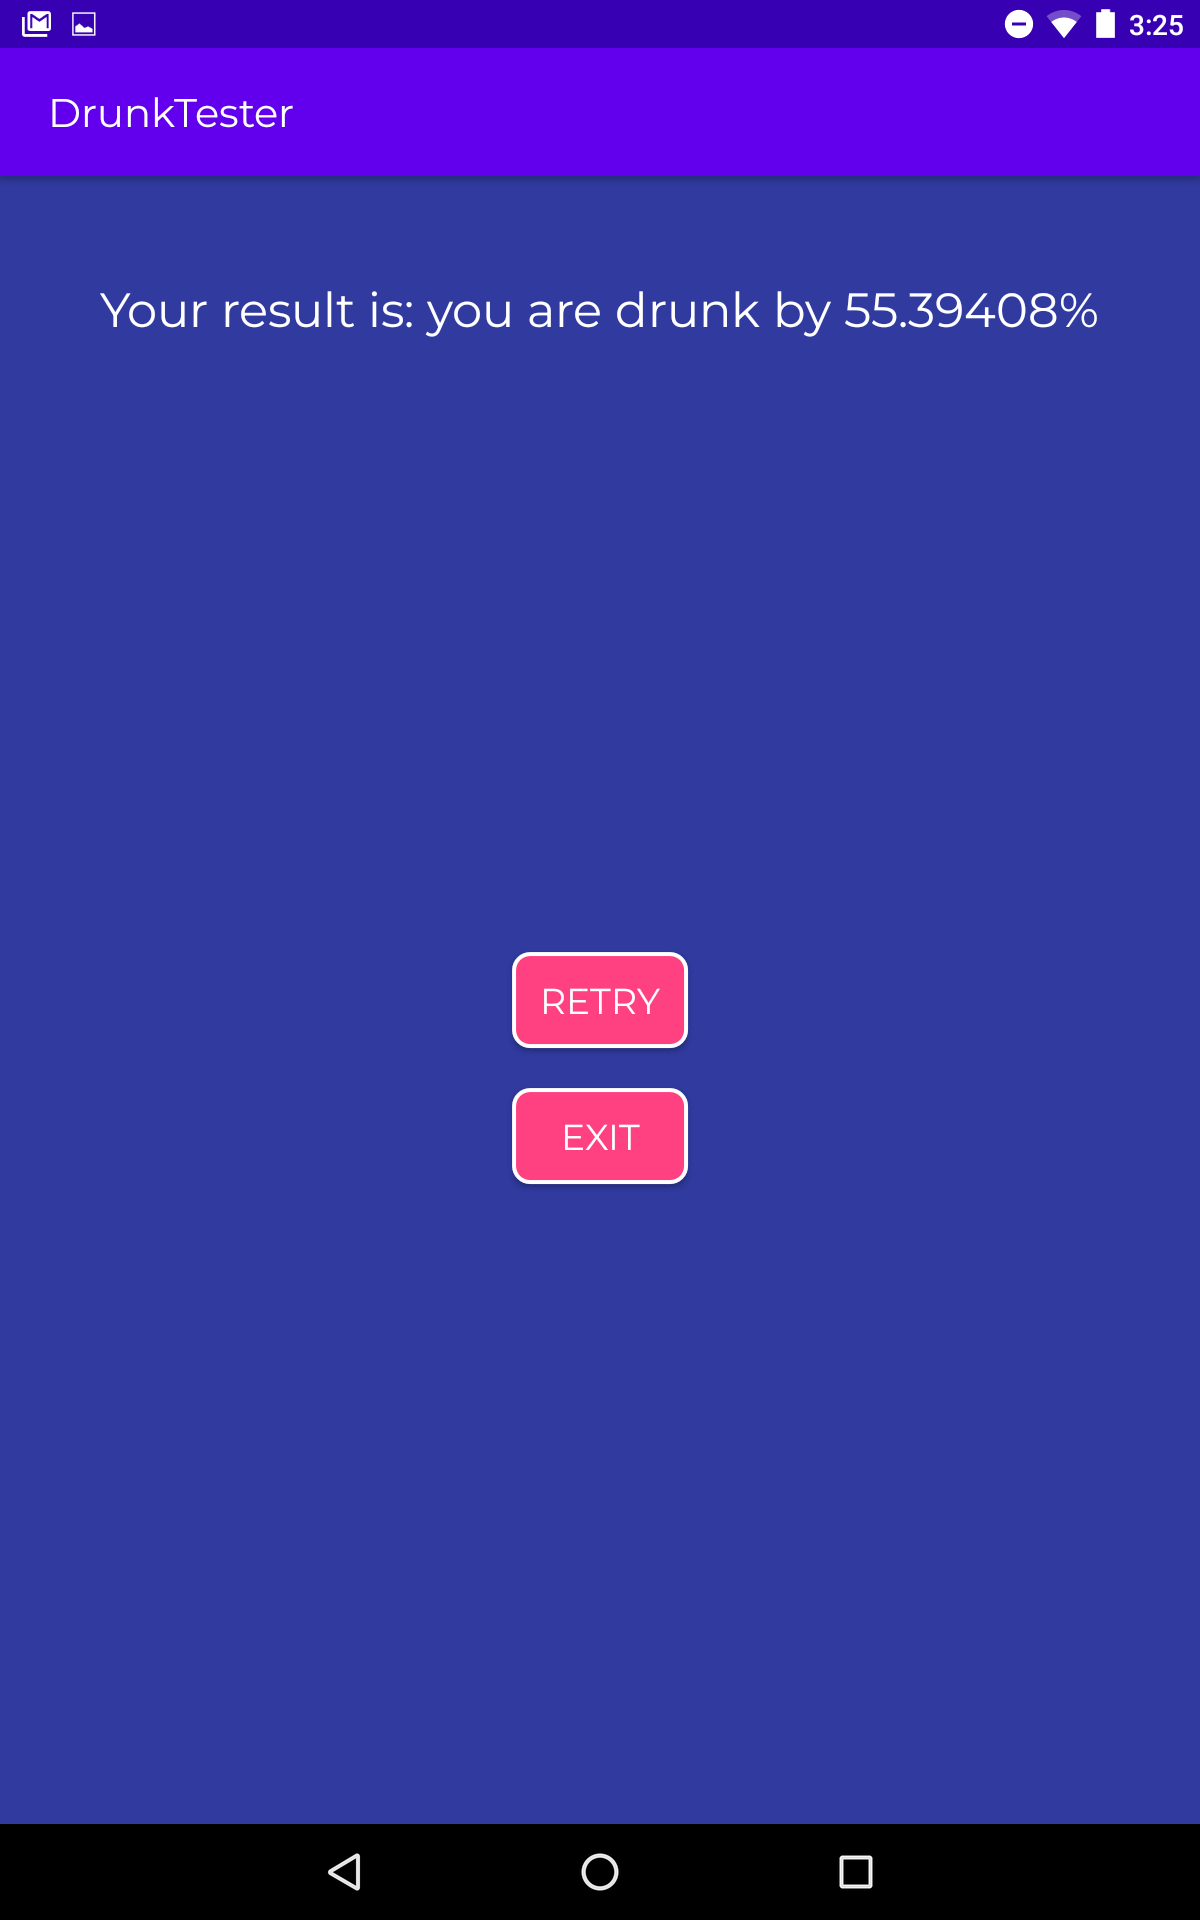
\includegraphics[width=\textwidth]{materials/Result_showcase_undetermined.png}
        \caption*{Result Showcase Undetermined: The screen displaying ~50\% result.}
    \end{subfigure}
    
    \caption*{Screenshots from the Drunk Tester application.}
\end{figure}

\newpage

\section{Implementation Details}

\begin{itemize}
    \item \textbf{Technologies Used:}
    \begin{itemize}
        \item \textbf{Android Studio:} Development environment.
        \item \textbf{Java:} Programming language for Android app.
        \item \textbf{JTransforms:} Library for performing FFT on voice data.
    \end{itemize}
    \item \textbf{Data Collection:}
    \begin{itemize}
        \item \textbf{Accelerometer:} Captures movement data.
        \item \textbf{Microphone:} Records voice.
    \end{itemize}
    \item \textbf{Data Analysis:}
    \begin{itemize}
        \item \textbf{Accelerometer:} Computes average acceleration and changes to determine stability.
        \item \textbf{Voice:} Applies FFT to analyze frequency components and compare power across frequency lanes.
    \end{itemize}
    \item \textbf{Algorithm:}
    \begin{itemize}
        \item Accelerometer data is analyzed using variance and rate of change.
        \item Voice data is processed using FFT to compute power in specified frequency lanes.
    \end{itemize}
\end{itemize}

\section{Code Overview}

\subsection{Class Descriptions}
\begin{itemize}
    \item \textbf{AccelerationAnalyzer.java} - Contains the class \texttt{AccelerationAnalyzer} which computes the probability of being drunk based on accelerometer data.
    \item \textbf{AccelerometerActivity.java} - Manages the accelerometer recording activity.
    \item \textbf{AnalyzeActivity.java} - Handles the analysis and display of results.
    \item \textbf{DataManager.java} - Manages the storage and retrieval of recorded data.
    \item \textbf{MainActivity.java} - The main entry point of the application.
    \item \textbf{RecordingAccelerometerActivity.java} - Records accelerometer data.
    \item \textbf{RecordingVoiceActivity.java} - Records voice data.
    \item \textbf{VoiceAnalyzer.java} - Analyzes the recorded voice data.
    \item \textbf{VoiceRecordActivity.java} - Manages the voice recording activity.
\end{itemize}

\subsection{Class and Method Descriptions}

\begin{longtable}{|p{5cm}|p{10cm}|}
\hline
\textbf{Class} & \textbf{Description} \\
\hline
\textbf{AccelerationAnalyzer-.java} & Contains methods to compute essential metrics from accelerometer data. \\
\hline
\textbf{Method} & \textbf{Description} \\
\hline
analyzeAcceleration-(List<float[ ]>) & Computes essentials passing the recorded data from accelerometers. \\
\hline
\end{longtable}

\begin{longtable}{|p{5cm}|p{10cm}|}
\hline
\textbf{Class} & \textbf{Description} \\
\hline
\textbf{AccelerometerActivity-.java} & Manages the activity for recording accelerometer data. \\
\hline
\textbf{Method} & \textbf{Description} \\
\hline
onCreate & Initializes the activity. \\
\hline
\end{longtable}

\begin{longtable}{|p{5cm}|p{10cm}|}
\hline
\textbf{Class} & \textbf{Description} \\
\hline
\textbf{AnalyzeActivity.java} & Handles the analysis of the recorded data. \\
\hline
\textbf{Method} & \textbf{Description} \\
\hline
onCreate & Initializes the activity. \\
analyzeData & Analyzes the collected accelerometer and voice data. \\
\hline
\end{longtable}

\begin{longtable}{|p{5cm}|p{10cm}|}
\hline
\textbf{Class} & \textbf{Description} \\
\hline
\textbf{DataManager.java} & Manages data storage and retrieval for the application. \\
\hline
\textbf{Method} & \textbf{Description} \\
\hline
DataManager & Constructor for initializing the DataManager. \\
getInstance & Returns the singleton instance of the DataManager. \\
setAccelerometerData & Sets the accelerometer data. \\
getAccelerometerData & Retrieves the accelerometer data. \\
setVoiceFileName & Sets the filename for the recorded voice data. \\
getVoiceFileName & Retrieves the filename for the recorded voice data. \\
clearData & Clears all stored data. \\
\hline
\end{longtable}

\begin{longtable}{|p{5cm}|p{10cm}|}
\hline
\textbf{Class} & \textbf{Description} \\
\hline
\textbf{MainActivity.java} & Main activity that initializes the application and checks permissions. \\
\hline
\textbf{Method} & \textbf{Description} \\
\hline
onCreate & Initializes the activity. \\
checkPermissions & Checks if the required permissions are granted. \\
onRequestPermissionsResult & Handles the result of the permission request. \\
\hline
\end{longtable}

\begin{longtable}{|p{5cm}|p{10cm}|}
\hline
\textbf{Class} & \textbf{Description} \\
\hline
\textbf{RecordingAccelerometer-Activity.java} & Manages the recording of accelerometer data. \\
\hline
\textbf{Method} & \textbf{Description} \\
\hline
onCreate & Initializes the activity. \\
startRecording & Starts the recording of accelerometer data. \\
run & Runnable for recording data at regular intervals. \\
stopRecording & Stops the recording of accelerometer data. \\
onSensorChanged & Handles sensor data changes. \\
onAccuracyChanged & Handles changes in sensor accuracy. \\
\hline
\end{longtable}

\begin{longtable}{|p{5cm}|p{10cm}|}
\hline
\textbf{Class} & \textbf{Description} \\
\hline
\textbf{RecordingVoice-Activity.java} & Manages the recording of voice data. \\
\hline
\textbf{Method} & \textbf{Description} \\
\hline
onCreate & Initializes the activity. \\
startRecording & Starts the recording of voice data. \\
run & Runnable for recording data at regular intervals. \\
stopRecording & Stops the recording of voice data. \\
\hline
\end{longtable}

\begin{longtable}{|p{5cm}|p{10cm}|}
\hline
\textbf{Class} & \textbf{Description} \\
\hline
\textbf{VoiceAnalyzer.java} & Analyzes the recorded voice data using FFT. \\
\hline
\textbf{Method} & \textbf{Description} \\
\hline
analyzeVoice & Analyzes the voice data using FFT. \\
readAudioFile & Reads the recorded audio file. \\
convertToDoubleArray & Converts audio data to a double array. \\
calculatePowerSpectrum & Calculates the power spectrum of the audio data. \\
analyzeFrequencyLanes & Analyzes the power in specified frequency lanes. \\
\hline
\end{longtable}

\begin{longtable}{|p{5cm}|p{10cm}|}
\hline
\textbf{Class} & \textbf{Description} \\
\hline
\textbf{VoiceRecordActivity.java} & Manages the voice recording activity. \\
\hline
\textbf{Method} & \textbf{Description} \\
\hline
onCreate & Initializes the activity. \\
\hline
\end{longtable}

\section{Data Analysis Details}

\subsection{Analyzing and Computing Accelerometer Data}

The listing of the computations related to this section will be followed in the Appendix A.
To visualize the overall computation, let's break it down into a flowchart or pseudocode:

1. \textbf{Compute Norm of Accelerometer Data:}
\[ xyzi[i] = \sqrt{x_i^2 + y_i^2 + z_i^2} \]


2. \textbf{Compute Rate of Change:}
\[ XYZ[0] = \frac{|xyzi[0] - xyzi[1]|}{\Delta} \]
\[ XYZ[i] = \frac{|xyzi[i-1] - 2 \times xyzi[i] + xyzi[i+1]|}{2 \times \Delta} \]
\[ XYZ[length - 1] = \frac{|xyzi[length - 2] - xyzi[length - 1]|}{\Delta} \]

3. \textbf{Compute Average Magnitude:}
\[ xyz\_avg = \frac{1}{length} \sum_{i=0}^{length-1} xyzi[i] \]

4. \textbf{Compute Final Result:}
\[ result = 100 \times \left( \frac{1}{1 + e^{-\tau \times (xyz\_avg - b)}} \right) \]

The parameters \( b \) and \( \tau \) are defined based on experimental data. The parameter \( b \) corresponds to the accumulated bias, while \( \tau \) determines the slope of the sigmoid function for a more responsive result.

\subsection{Analyzing and Computing Voice Data}

Just as with the previous subsection, the listing related to this part is provided in Appendix B.
The process involves applying Fourier transformation to analyze the voice in the frequency space.

1. \textbf{Fourier Transform:}
\[ A[k] = \sum_{n=0}^{N-1} a[n] e^{-2\pi ikn/N} \]

2. \textbf{Power Spectrum:}
\[ P[k] = (\text{Re}(A[k]))^2 + (\text{Im}(A[k]))^2 \]

3. \textbf{Frequency Lanes:}
\[ \text{Lanes} = \{ [60, 90], [90, 120], \ldots, [270, 300] \} \]

4. \textbf{Power in Lanes:}
\[ P_{\text{lane}_i} = \sum_{k=f_{\text{start}}}^{f_{\text{end}}} P[k] \]

5. \textbf{Result Calculation:}
\[ \text{Result} = \left\{
\begin{array}{ll}
1 & \text{if Count} \geq 5 \\
0.8 & \text{if Count} = 4 \\
0.75 & \text{if Count} = 3 \\
0.5 & \text{if Count} = 2 \\
0 & \text{otherwise}
\end{array} \right. \]

\section{Inferences and Future Improvements}

The parameters for the acceleration activity, \( b \) and \( \tau \), are defined based on experiments. The parameter \( b \) corresponds to the accumulated bias due to the nature of accelerometers, which always have some motion and record an approximate bias of 9.8. The parameter \( \tau \) changes the slope of the sigmoid function to make the result more responsive to changes in acceleration.

The current version of the application computes the result as a weighted average of the accelerometer and voice data results, with weights of 0.8 and 0.2, respectively. This weighting may need adjustment based on further testing.

Future improvements include dynamically adjusting the sound frequency bandwidth lanes for less discrete analysis and further tuning the parameters for more accurate results.

\section*{References}
\begin{enumerate}
    \item \textbf{Mamanchuk N., University of Tsukuba}, DrunkTester Project for Android - Github, \today. Available online: \url{https://github.com/RIFLE/IoT-Projects}
\end{enumerate}

\newpage

\section*{Appendix A. Listing AccelerationAnalyzer.java}

The following code is the implementation of the class which provides a method analyzeAcceleration() to compute a result for the correspondingly recorded data.

\vspace{5mm}

\begin{lstlisting}
public class AccelerationAnalyzer {

public static float analyzeAcceleration(List<float[]> accelerometerData) {

        double b = 9.805;
        double tau = 22.67;

        double[] xyzi = new double[accelerometerData.size()];
        for (int i = 0; i < accelerometerData.size(); i++) {
            float x = accelerometerData.get(i)[0];
            float y = accelerometerData.get(i)[1];
            float z = accelerometerData.get(i)[2];
            xyzi[i] = Math.sqrt(x * x + y * y + z * z);
        }

        // Compute the rate of change
        double[] XYZ = new double[xyzi.length];
        double delta = 0.1;
        XYZ[0] = Math.abs(xyzi[0] - xyzi[1]) / delta;
        for (int i = 1; i < xyzi.length - 1; i++) {
            XYZ[i] = Math.abs(xyzi[i - 1] - 2 * xyzi[i] + xyzi[i + 1]) / (2 * delta);
        }
        XYZ[xyzi.length - 1] = Math.abs(xyzi[xyzi.length - 2] - xyzi[xyzi.length - 1]) / delta;

        // Compute the average modulus of momentary acceleration
        double xyz_avg = 0;
        for (double xyz : xyzi) {
            xyz_avg += xyz;
        }
        xyz_avg /= xyzi.length;



        // Compute the result
        return (float) (100 * (1 / (1 + Math.exp(- tau * (xyz_avg - b)))));
}
\end{lstlisting}

\newpage

\section*{Appendix B. Listing VoiceAnalyzer.java}

Similarly to the previously defined we provide the listing for analyzing voice data.

\vspace{5mm}

\begin{lstlisting}
    public class VoiceAnalyzer {

    public static float analyzeVoice(String voiceFileName) {
        try {
            // Read the audio file
            byte[] audioBytes = readAudioFile(voiceFileName);

            // Convert bytes to double for FFT
            double[] audioData = convertToDoubleArray(audioBytes);

            // Perform FFT
            DoubleFFT_1D fft = new DoubleFFT_1D(audioData.length);
            fft.realForward(audioData);

            // Calculate power spectrum
            double[] powerSpectrum = calculatePowerSpectrum(audioData);

            // Analyze power in specified frequency lanes
            return analyzeFrequencyLanes(powerSpectrum);

        } catch (IOException e) {
            e.printStackTrace();
            return 0;
        }
    }

    private static byte[] readAudioFile(String voiceFileName) throws IOException {
        File file = new File(voiceFileName);
        FileInputStream fis = new FileInputStream(file);
        byte[] data = new byte[(int) file.length()];
        fis.read(data);
        fis.close();
        return data;
    }

    private static double[] convertToDoubleArray(byte[] audioBytes) {
        double[] audioData = new double[audioBytes.length];
        for (int i = 0; i < audioBytes.length; i++) {
            audioData[i] = (double) audioBytes[i];
        }
        return audioData;
    }

    private static double[] calculatePowerSpectrum(double[] audioData) {
        int n = audioData.length / 2;
        double[] powerSpectrum = new double[n];
        for (int i = 0; i < n; i++) {
            double real = audioData[2 * i];
            double imag = audioData[2 * i + 1];
            powerSpectrum[i] = Math.sqrt(real * real + imag * imag);
        }
        return powerSpectrum;
    }

    private static float analyzeFrequencyLanes(double[] powerSpectrum) {
        int sampleRate = 44100; // Change if your sample rate is different
        int n = powerSpectrum.length;

        // Frequency resolution
        double freqResolution = (double) sampleRate / n;

        // Define lanes
        int[] lanes = {60, 90, 120, 150, 180, 210, 240, 270, 300};
        double[] lanePowers = new double[lanes.length - 1];

        // Calculate power in each lane
        for (int i = 0; i < lanes.length - 1; i++) {
            int startFreq = lanes[i];
            int endFreq = lanes[i + 1];
            int startIndex = (int) (startFreq / freqResolution);
            int endIndex = (int) (endFreq / freqResolution);

            for (int j = startIndex; j < endIndex; j++) {
                lanePowers[i] += powerSpectrum[j];
            }
        }

        // Find the most powerful lane
        double maxPower = 0;
        for (double power : lanePowers) {
            if (power > maxPower) {
                maxPower = power;
            }
        }

        double centralLanePower = 0;
        int centralLaneIndex = 0;

        for (int i = 0; i < lanePowers.length; i++) {
            if (lanePowers[i] == maxPower) {
                centralLanePower = lanePowers[i];
                centralLaneIndex = i;
                break;
            }
        }

        // Compare power of other lanes with the central lane
        int count = 0;
        for (int i = 0; i < lanePowers.length; i++) {
            if (i != centralLaneIndex && lanePowers[i] >= 0.75 * centralLanePower) {
                count++;
            }
        }

        // Calculate the result
        if (count >= 5) {
            return 1;
        } else if (count == 4) {
            return 0.8f;
        } else if (count == 3) {
            return 0.75f;
        } else if (count == 2) {
            return 0.5f;
        } else {
            return 0;
        }
    }
}
\end{lstlisting}

\end{document}
